\documentclass[12pt]{article}
\usepackage{amsmath,amssymb}
\usepackage{graphicx}
\usepackage{authblk}
\usepackage{geometry}
\usepackage{cite}
\geometry{margin=1in}

\title{DRAFT -- Recursive Scalar Field Dynamics in Loop Quantum Cosmology: \\
Attractor Emergence Across Cosmological Bounces}
\author{Nicholas Parian}
\affil{Independent Researcher}
\date{\today}

\begin{document}

\maketitle

\begin{abstract}
We present a simplified cosmological model within the framework of Loop Quantum Cosmology (LQC) in which scalar field dynamics evolve recursively across universe bounce cycles. We demonstrate that under damping and bounded potentials, these dynamics converge to attractor states in phase space. This attractor behavior suggests an effective memory mechanism across cosmic epochs, offering a new perspective on informational persistence and structure emergence in bouncing universes. We outline testable predictions relevant to CMB anomalies and low-entropy configurations.
\end{abstract}

\section{Introduction}

Standard cosmological models based on general relativity predict an initial singularity—a breakdown of physics at the beginning of time. Loop Quantum Cosmology (LQC) offers a resolution by replacing this singularity with a quantum bounce\cite{Ashtekar2006,Agullo2017,Bojowald2008}, allowing the universe to evolve smoothly through classically forbidden regimes. While LQC has been studied extensively in the context of singularity resolution and inflationary dynamics, the question of whether any structure or information persists across bounces remains underexplored.

This work investigates whether scalar field evolution under LQC dynamics exhibits attractor behavior across cycles. Attractors in phase space represent dynamically stable configurations toward which a system converges regardless of initial conditions. We show that under damping and bounded potentials, scalar fields in LQC naturally evolve toward such states, forming a kind of memory across cosmic epochs. This mechanism provides a new angle on the emergence of order and the recurrence of low-entropy conditions after each bounce—without invoking quantum coherence between cycles.

We propose that these attractors could leave observable imprints on the cosmic microwave background and inflationary initial conditions, and offer a deterministic, classical alternative to probabilistic quantum interpretations of cosmic structure formation.

\section{Theoretical Framework}

\subsection{Loop Quantum Cosmology Basics}

In standard cosmology, the Friedmann equation describes how the expansion rate of the universe depends on its energy content. LQC modifies this by incorporating quantum gravity corrections, leading to a repulsive effect near Planck-scale densities. The modified Friedmann equation reads:

\begin{equation}
H^2 = \frac{8\pi G}{3} \rho \left(1 - \frac{\rho}{\rho_c}\right)
\end{equation}

Here, $H$ is the Hubble parameter, $\rho$ is the total energy density, and $\rho_c$ is a critical density—typically on the order of the Planck density—above which quantum gravitational effects dominate. When $\rho = \rho_c$, the expansion rate vanishes ($H = 0$), causing a bounce that replaces the classical singularity.

\subsection{Scalar Field Dynamics}

The evolution of a scalar field $\phi$ in an expanding universe follows the Klein-Gordon equation:

\begin{equation}
\ddot{\phi} + 3H\dot{\phi} + \frac{dV}{d\phi} = 0
\end{equation}

The second term acts as a friction term proportional to the Hubble rate. The scalar field's energy density contributes to $\rho$ via:

\[
\rho = \frac{1}{2}\dot{\phi}^2 + V(\phi)
\]\cite{Mukhanov2005}

We examine two representative potentials:

\begin{itemize}
  \item \textbf{Quadratic:} $V(\phi) = \frac{1}{2}m^2\phi^2$ — a simple harmonic potential.
  \item \textbf{Periodic:} $V(\phi) = \Lambda^4[1 - \cos(\phi/f)]$ — a bounded, multi-well potential often associated with axion physics\cite{Marsh2016}.
\end{itemize}

Both potentials are bounded from below and admit oscillatory behavior. When combined with damping from the expansion term and the bounce-induced dynamics, these potentials support long-term convergence of trajectories toward attractor states in phase space.


\section{Attractor Convergence Model}

We model the evolution of the universe through successive bounce cycles by defining a discrete state vector:

\begin{equation}
U_n = (\phi_n, \dot{\phi}_n, \rho_n)
\end{equation}

This state evolves deterministically via a recurrence relation:

\begin{equation}
U_{n+1} = T(U_n)
\end{equation}

where \(T\) is the transformation applied over one bounce-expansion-contraction cycle. We impose a phenomenological damping condition across cycles, implemented as:

\begin{equation}
\dot{\phi}_{n+1} = \gamma \dot{\phi}_n
\end{equation}

with \(0 < \gamma < 1\), representing energy loss due to bounce-induced friction, expansion drag, or other coarse-grained dissipative effects. Combined with the scalar potential’s restoring force, the system evolves toward a constrained subset of phase space.

In the case of a quadratic potential, this leads to a fixed point at \((\phi, \dot{\phi}) = (0, 0)\). In the periodic potential, convergence occurs to one of the potential minima, forming a stable oscillatory orbit. In both scenarios, trajectories from a wide range of initial conditions spiral into attractor structures.

This attractor behavior is not due to quantum interference or probabilistic branching but instead emerges from deterministic recursive dynamics under dissipation. It offers a classical mechanism for phase space contraction and structural persistence across cosmic cycles.


\section{Simulation Results}

We simulate scalar field evolution through bounce cycles using numerical integration of the modified Friedmann and Klein-Gordon equations. Each simulation includes LQC bounce dynamics, damping, and (optionally) stochastic noise. Initial conditions and parameters are chosen to explore both single-field and multi-field configurations under quadratic and periodic potentials. Tracking the total energy density across time steps shows sharp peaks at each bounce when $\rho = \rho_c$, followed by decline due to dissipation. This validates that bounces are correctly triggered by LQC constraints\cite{Ashtekar2006} and that damping mechanisms reduce system energy across cycles.


\begin{figure}[h]
  \centering
  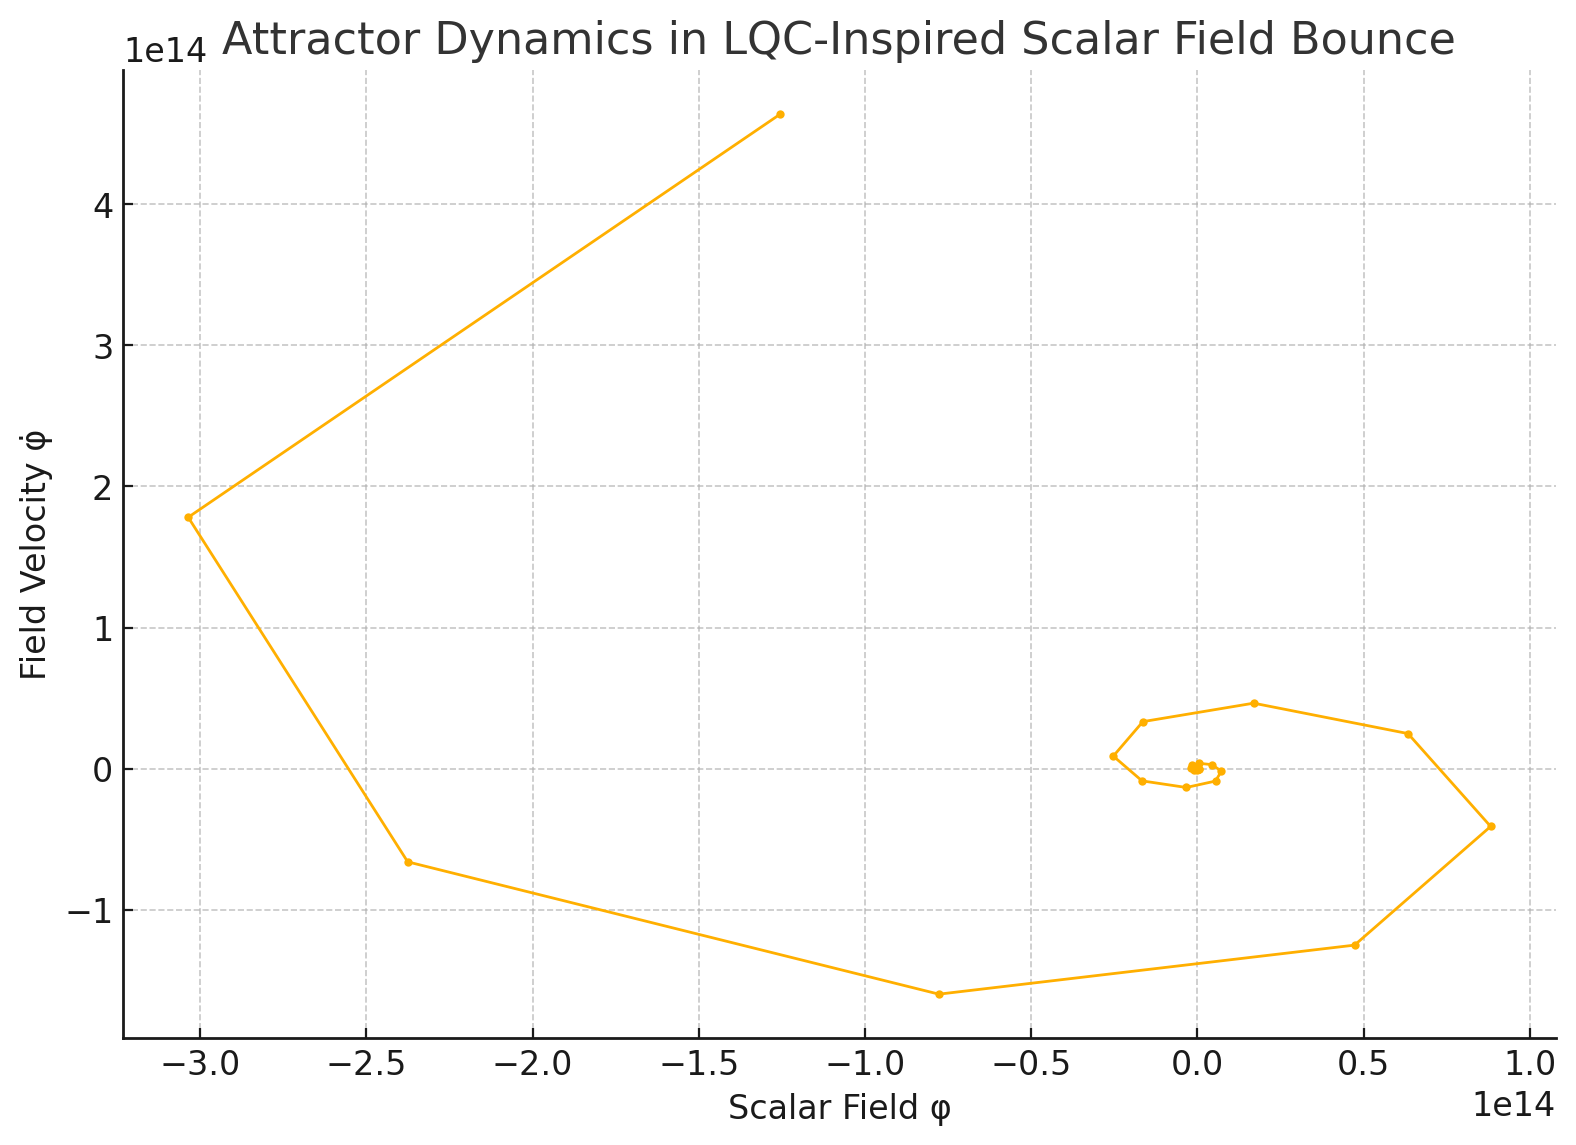
\includegraphics[width=0.7\textwidth]{figures/quadratic_attractor.png}
  \caption{Phase space trajectory in the quadratic potential $V(\phi) = \frac{1}{2}m^2\phi^2$. The system exhibits spiral convergence toward $(\phi, \dot{\phi}) = (0, 0)$ under damping.}
\end{figure}

In the quadratic potential, the scalar field undergoes damped oscillations. The trajectory in $(\phi, \dot{\phi})$ phase space forms a shrinking spiral converging to the origin. This fixed-point attractor demonstrates exponential memory loss of initial conditions and phase space volume contraction over cycles.

\begin{figure}[h]
  \centering
  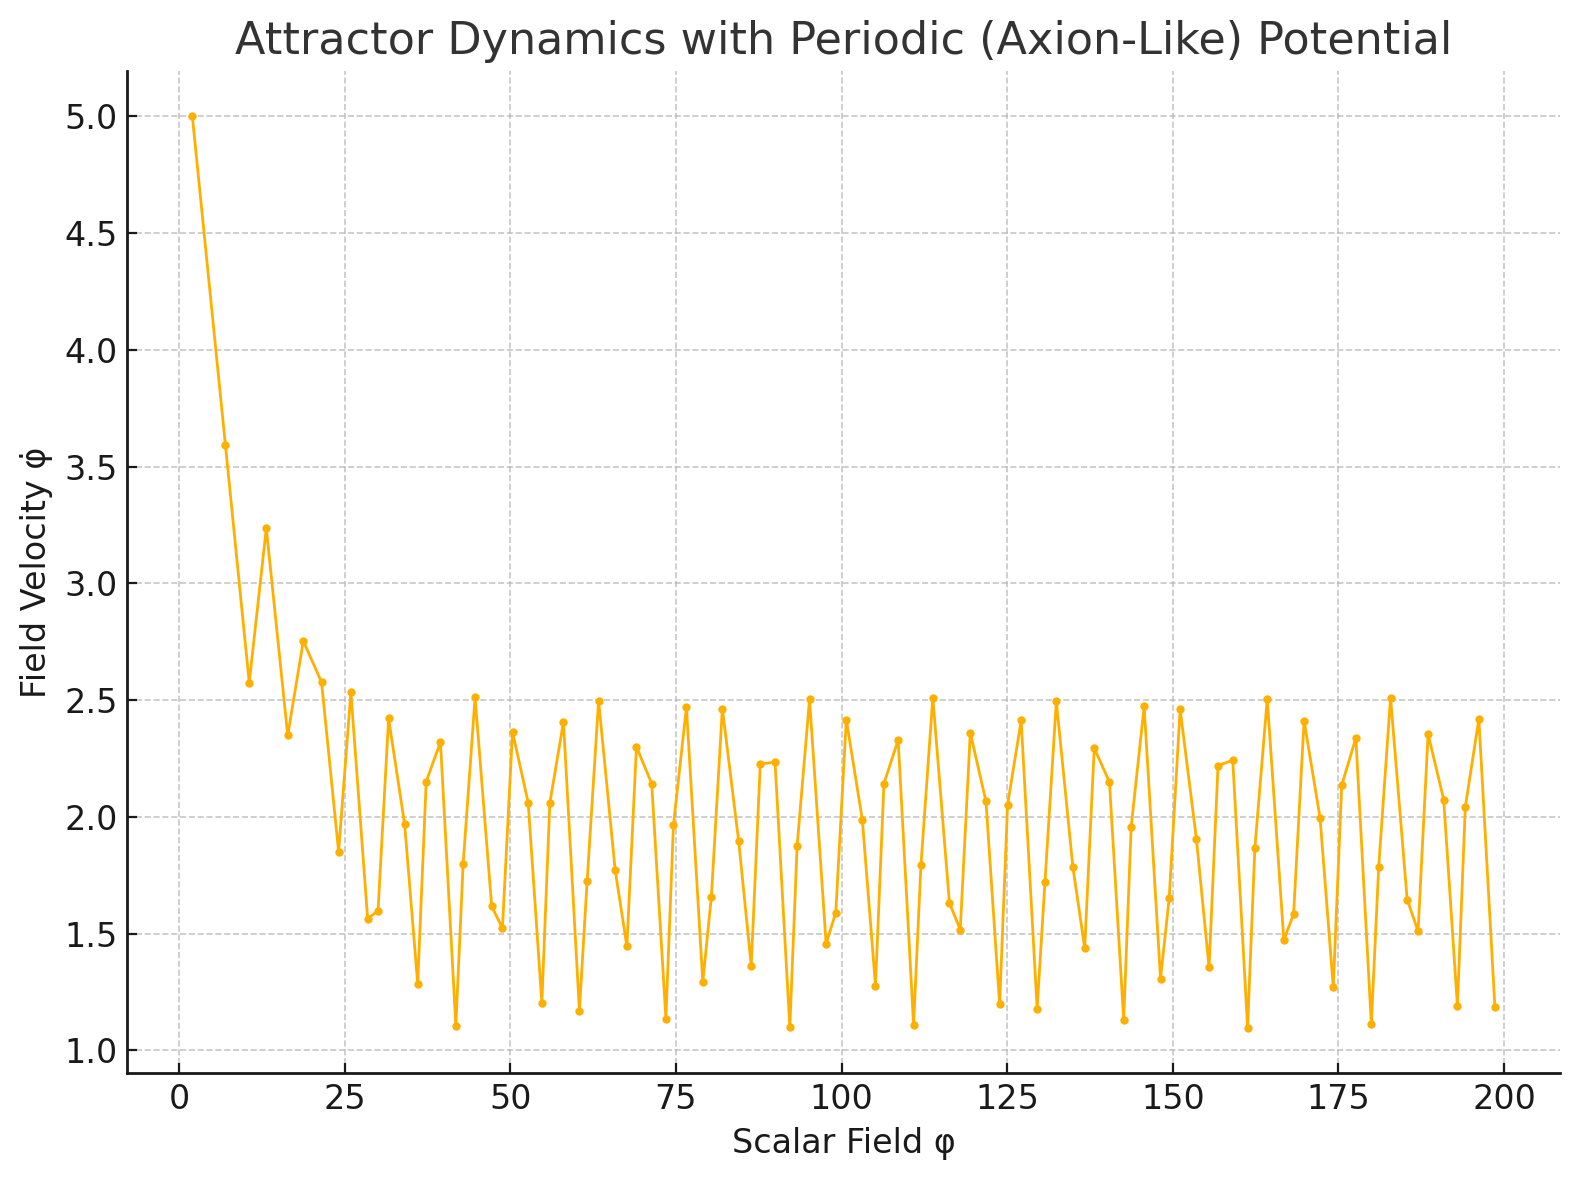
\includegraphics[width=0.7\textwidth]{figures/periodic_attractor.png}
  \caption{Phase space spiral with periodic (axion-like) potential $V(\phi) = \Lambda^4[1 - \cos(\phi/f)]$.}
\end{figure}

In the periodic potential, the scalar field experiences damped oscillations within a bounded multi-well landscape. Instead of converging to a single point, the system settles into a stable orbit near one of the cosine minima. This forms a limit cycle attractor, whose location depends on initial conditions but whose structure is robust under bounce dynamics.

\begin{figure}[h]
  \centering
  \includegraphics[width=0.7\textwidth]{figures/total_energy_density.png}
  \caption{Total energy density $\rho$ as a function of simulation time. The bounce occurs when $\rho$ reaches $\rho_c$. Post-bounce damping reduces energy in each cycle.}
\end{figure}

Tracking the total energy density across time steps shows sharp peaks at each bounce when $\rho = \rho_c$, followed by decline due to dissipation. This validates that bounces are correctly triggered by LQC constraints and that damping mechanisms reduce system energy across cycles.

\begin{figure}[h]
  \centering
  \includegraphics[width=0.7\textwidth]{figures/3d_phase_space_uncoupled.png}
  \caption{3D phase space trajectory in $(\phi, \dot{\phi}, \chi)$ with bounce and quantum noise, but no field interaction coupling.}
\end{figure}

In a two-field system with a second scalar field $\chi$ governed by an independent periodic potential, the full phase space becomes multidimensional. Even with quantum noise, trajectories converge toward bounded regions in the $(\phi, \dot{\phi}, \chi)$ manifold—demonstrating multi-field attractor formation without coupling.

\begin{figure}[h]
  \centering
  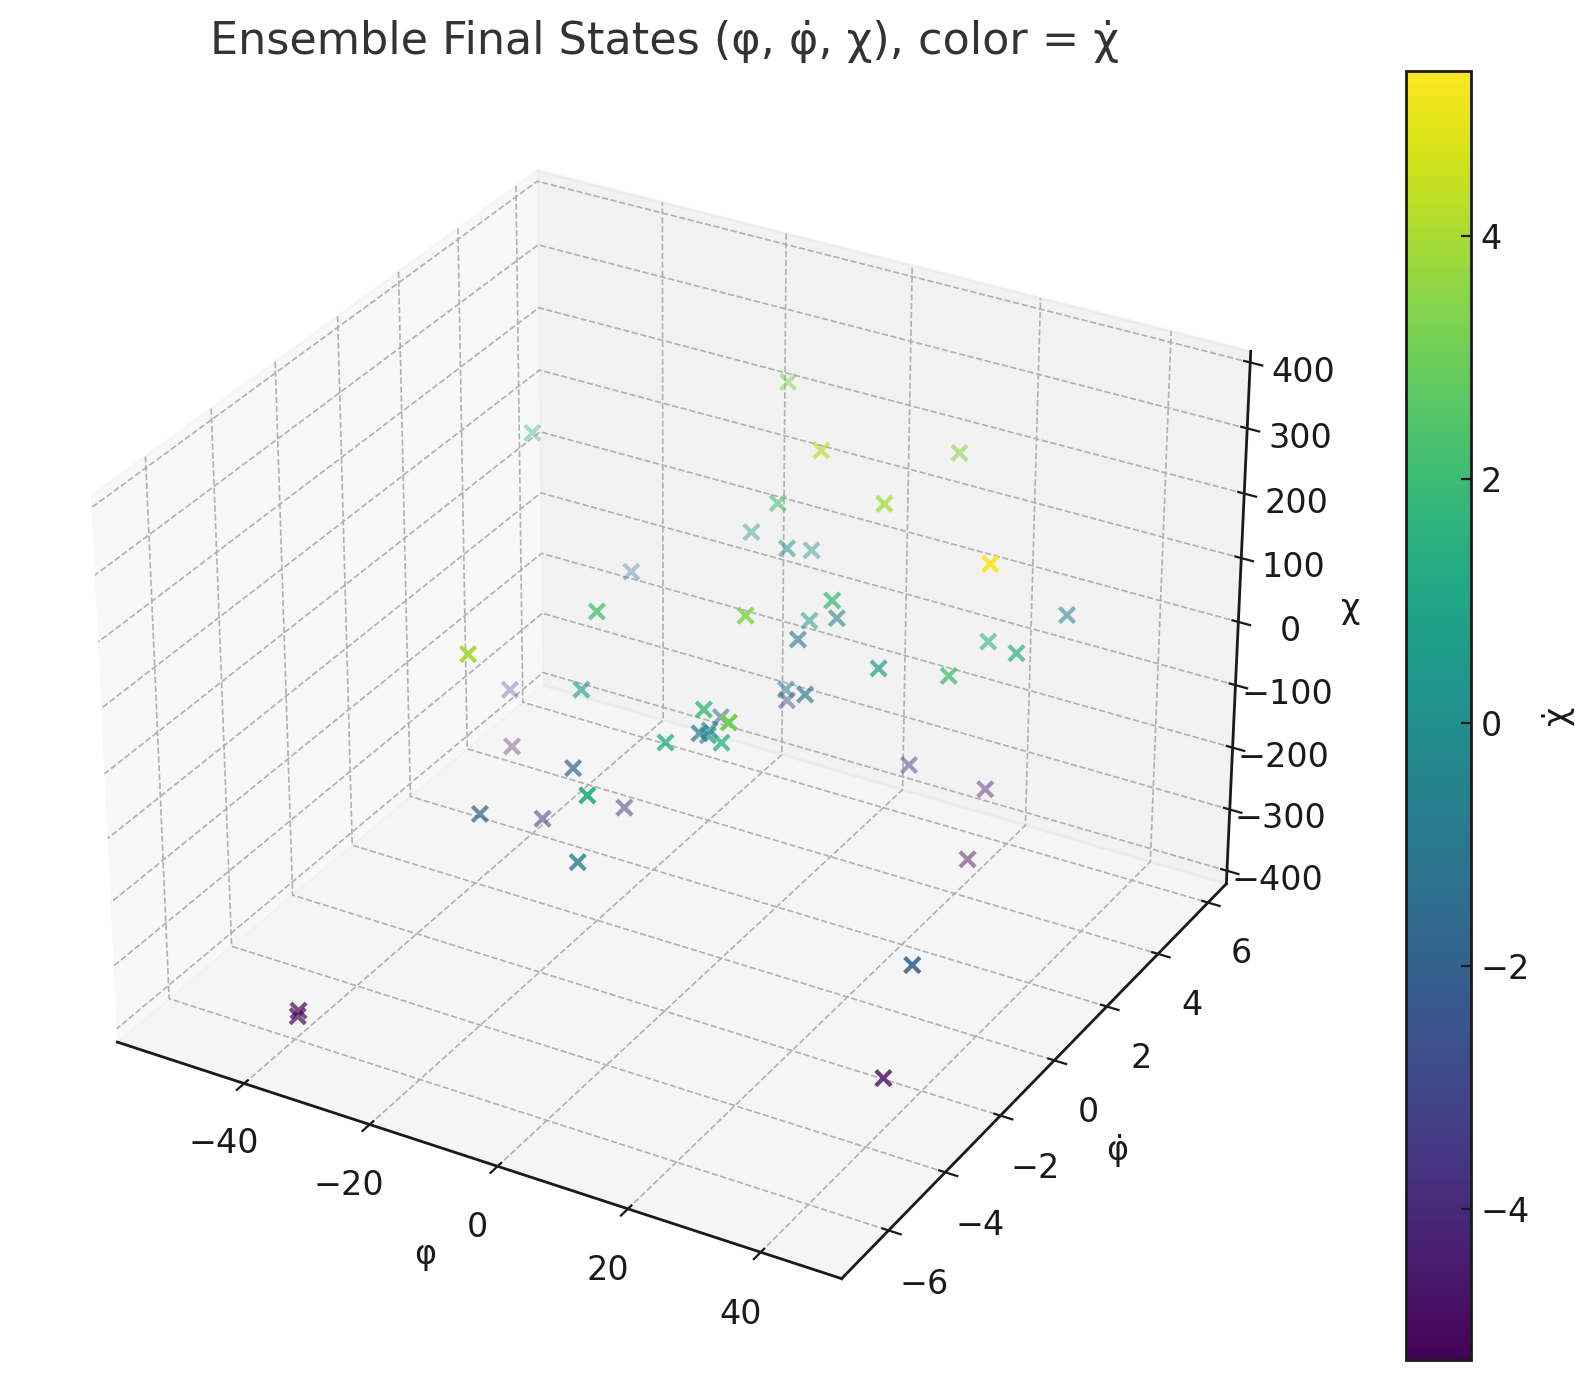
\includegraphics[width=0.7\textwidth]{figures/ensemble_attractor_cloud.png}
  \caption{Final state ensemble distribution across random initial conditions. The bounded cloud reflects probabilistic attractor convergence.}
\end{figure}

To assess the statistical nature of attractor behavior, we simulate 50 universes with randomized initial conditions and noise. The final states form a compact cloud in $(\phi, \dot{\phi}, \chi)$ space. The structure resembles a classical analogue of an interference pattern: high-density convergence zones surrounded by sparse outliers. This demonstrates that deterministic recursion under LQC filtering selects bounded outcomes even under stochastic perturbation.

These simulations show that scalar field evolution in LQC consistently leads to attractor formation under a wide range of conditions. Whether operating in single-field or two-field configurations, and whether the potential is quadratic or periodic, recursive damping and bounce mechanics guide the system toward dynamically stable regions of phase space. Crucially, the attractors persist even under the influence of quantum noise and randomized starting conditions, indicating structural robustness.

The resulting attractor structures function as a classical mechanism for filtering cosmological degrees of freedom. Rather than diffusing or amplifying initial condition variance, the system recursively contracts the phase space volume of viable configurations. This provides a new pathway for understanding how low-entropy, structured universes could re-emerge after each bounce—offering an alternative to explanations rooted in quantum cosmological interference.

\section{Observable Predictions}

If attractor structures are a generic outcome of scalar field dynamics in LQC, they should produce observable consequences in the structure and evolution of our universe. These predictions follow directly from the contraction of phase space volume and the recurrence of bounded configurations across cycles.
Recursive filtering reduces the effective number of degrees of freedom. This could manifest as low-variance zones, cold spots, or other entropy-suppressing features at large angular scales—similar to anomalies observed by WMAP and Planck\cite{Planck2020}. The resulting scalar field distribution should be statistically distinguishable from models that assume broad, randomly seeded inflationary states\cite{Remmen2013,Carroll2005}.



\begin{itemize}
  \item \textbf{Preferred inflationary initial states:} Attractor convergence implies that the inflaton field enters the inflationary phase from a narrow region of phase space. This constraint would limit the range of inflationary trajectories and affect the expected distribution of e-folds and perturbation spectra.

  \item \textbf{Low-entropy anomalies in the CMB:} Recursive filtering reduces the effective number of degrees of freedom. This could manifest as low-variance zones, cold spots, or other entropy-suppressing features at large angular scales—similar to anomalies observed by WMAP and Planck.

  \item \textbf{Recurrent angular patterns:} If post-bounce configurations repeatedly collapse into similar attractor wells, the geometry of early-universe perturbations could reflect non-random correlations across cycles—possibly visible as subtle symmetries in CMB angular power.

  \item \textbf{Phase space suppression signatures:} Over successive bounces, the attractor mechanism effectively prunes the allowed configuration space. The resulting scalar field distribution should be statistically distinguishable from models that assume broad, randomly seeded inflationary states.
\end{itemize}

These features—especially suppression of entropy, reduction in field variability, and structured anomalies in large-scale CMB data—could provide indirect evidence for recursive attractor formation in bounce cosmologies. High-resolution data from upcoming missions like CMB-S4 may be able to detect or falsify such predictions.

\section{Discussion}

This work demonstrates that attractor behavior in scalar field dynamics arises naturally within Loop Quantum Cosmology under minimal assumptions: damping, bounded potentials, and bounce recursion. These attractors function as dynamic memory structures, guiding the evolution of field configurations toward constrained regions of phase space regardless of initial conditions.

This convergence provides a deterministic mechanism for post-bounce structure and entropy suppression—without invoking quantum coherence, wavefunction collapse, or exotic cyclic metaphysics. In contrast to chaotic or diffusive cosmological models, attractor filtering selects for predictability and recurrence. The emergence of order is a consequence of dynamics, not assumption.

A rigorous model would derive dissipation from quantum backreaction or effective field theory\cite{Bojowald2008}.


However, the current model is highly idealized. Key limitations include:

\begin{itemize}
  \item \textbf{Homogeneous fields only:} We neglect spatial perturbations and anisotropies, which are critical in realistic cosmology.
  \item \textbf{Phenomenological damping:} The damping factor $\gamma$ is inserted by hand. A rigorous model would derive dissipation from quantum backreaction or effective field theory.
  \item \textbf{No metric backreaction:} Geometry evolves independently of field fluctuations; true semiclassical dynamics would require coupling between matter and geometry.
  \item \textbf{Semiclassical approximation:} Quantum fluctuations and decoherence effects are not explicitly modeled.
\end{itemize}

Despite these simplifications, the results suggest that attractor formation is a robust and potentially generic feature of bouncing cosmologies. Future extensions should incorporate field perturbations, quantized fluctuations, metric-field coupling, and more realistic potentials. Statistical comparisons with cosmological datasets could help determine whether attractor convergence leaves detectable imprints.

Ultimately, this attractor mechanism offers a new approach to the question of how low-entropy, structured universes emerge from bounce dynamics—without needing to appeal to fine-tuned initial conditions or many-worlds explanations.
\section{Conclusion}

We have presented a simplified yet powerful model in which scalar fields evolving under Loop Quantum Cosmology exhibit convergence toward attractor states across multiple bounce cycles. These attractors arise from the interplay of damping, bounded potentials, and bounce-induced recursions. Our simulations show that such behavior persists even in the presence of quantum noise and stochastic perturbations.

These attractors act as dynamical memory structures—selecting, stabilizing, and constraining field evolution in a way that naturally filters phase space and suppresses entropy. This provides a deterministic, classical mechanism for the recurrence of structure in a cyclic universe—one that does not rely on quantum interference, anthropic reasoning, or fine-tuned initial conditions.

We propose that attractor-based models may produce observable signatures in inflationary dynamics and the cosmic microwave background. In particular, we suggest looking for signs of entropy suppression, preferred inflationary onset states, and non-random correlations across large angular scales.

This work offers a new paradigm for cosmological recurrence: not one of perfect reset or many-worlds branching, but of progressive convergence. The emergence of order across cycles may be a natural feature of the universe’s own dynamics.

\begin{thebibliography}{99}

\bibitem{Ashtekar2006}
Ashtekar, A., Pawlowski, T., \& Singh, P. (2006). Quantum nature of the big bang: Improved dynamics. \textit{Phys. Rev. D}, 74(8), 084003.

\bibitem{Agullo2017}
Agullo, I., \& Singh, P. (2017). Loop Quantum Cosmology: A brief review. \textit{arXiv preprint} arXiv:1612.01236 [gr-qc].

\bibitem{Bojowald2008}
Bojowald, M. (2008). Loop quantum cosmology. \textit{Living Reviews in Relativity}, 11(1), 4.

\bibitem{Liddle2000}
Liddle, A. R., \& Lyth, D. H. (2000). \textit{Cosmological Inflation and Large-Scale Structure}. Cambridge University Press.

\bibitem{Kaiser1995}
Kaiser, D. I. (1995). Primordial spectral indices from generalized Einstein theories. \textit{Phys. Rev. D}, 52(8), 4295.

\bibitem{Remmen2013}
Remmen, G. N., \& Carroll, S. M. (2013). How many e-folds should we expect from high-scale inflation? \textit{Phys. Rev. D}, 88(8), 083518.

\bibitem{Planck2020}
Planck Collaboration. (2020). Planck 2018 results. VII. Isotropy and statistics of the CMB. \textit{Astronomy \& Astrophysics}, 641, A7.

\bibitem{Carroll2005}
Carroll, S. M. (2005). Why is there something, rather than nothing? The entropy argument for cosmological initial conditions. \textit{arXiv preprint} hep-th/0505037.

\bibitem{Penrose2010}
Penrose, R. (2010). \textit{Cycles of Time: An Extraordinary New View of the Universe}. The Bodley Head.

\bibitem{Freese1990}
Freese, K., Frieman, J. A., \& Olinto, A. V. (1990). Natural inflation with pseudo–Nambu-Goldstone bosons. \textit{Phys. Rev. Lett.}, 65(26), 3233.

\bibitem{Marsh2016}
Marsh, D. J. E. (2016). Axion cosmology. \textit{Phys. Rept.}, 643, 1–79.

\bibitem{Achucarro2011}
Achúcarro, A., Gong, J.-O., Hardeman, S., Palma, G. A., \& Patil, S. P. (2011). Features of heavy physics in the CMB power spectrum. \textit{JCAP}, 2011(01), 030.

\bibitem{Bardeen1983}
Bardeen, J. M., Steinhardt, P. J., \& Turner, M. S. (1983). Spontaneous creation of almost scale-free density perturbations in an inflationary universe. \textit{Phys. Rev. D}, 28(4), 679.

\bibitem{Mukhanov2005}
Mukhanov, V. F. (2005). \textit{Physical Foundations of Cosmology}. Cambridge University Press.

\end{thebibliography}

\section*{Acknowledgments}
The author acknowledges the use of OpenAI's ChatGPT-4o model for formatting support, LaTeX editing, and reference management, and contributions.



\end{document}